\chapter{Algoritmos de Referencia}

En este capítulo se presentan los dos algoritmos que se utilizaran como base para desarrollar un algoritmo competitivo para problemas \textit{expensive}, se describirán con sus referencias y se indicarán algunas características; aunque se explicarán de forma más detallada los componentes propios de cada uno en el siguiente capítulo.

\section{Algoritmo Genético Estacionario Uniforme}

En primer lugar, debemos explicar brevemente la importancia de los Algoritmos Genéticos (AG) y, posteriormente, justificar la elección de su versión Algoritmo Genético Estacionario Uniforme (AGEU). 

Los seres vivos son solucionadores de problemas de forma natural. 
Exhiben una versatilidad que ponen en evidencia hasta a los mejores programas. 
Esta observación es especialmente humillante para los informáticos, que necesitan utilizar meses e incluso años de esfuerzos intelectuales en un algoritmo, mientras que estos organismos obtienen sus habilidades a través de los aparentemente indirectos mecanismos de evolución y selección natural. 

Los investigadores más pragmáticos observan el notable poder de la evolución como algo que simular. 
La selección natural elimina uno de los mayores inconvenientes en el diseño de software: especificar de antemano todas las características de un problema y las acciones que dicho programa tendría que tomar para tratar con ellas. 
Aprovechando los mecanismos de evaluación, los investigadores pueden ser capaces de ``reproducir'' programas que resuelvan problemas incluso cuando nadie pueda comprender enteramente su estructura. 
Efectivamente, estos llamados \textbf{algoritmos genéticos} han demostrado la habilidad de hacer avances en el diseño de sistemas complejos. 

Los AGs hacen posible explorar un rango mucho más amplio de posibles soluciones a un problema que programas convencionales. 
Además, en los estudios  realizados sobre la selección natural de programas bajo condiciones controladas bien entendidas, los resultados prácticos alcanzados pueden aportar cierto conocimiento sobre los detalles de cómo la vida y la inteligencia evolucionan en el mundo natural. 

El funcionamiento de un AG viene dado por el siguiente pseudocódigo (Algoritmo \ref{alg:AG})

\begin{algorithm}
\caption{Algoritmo Genético}\label{alg:AG}
\begin{algorithmic}[1]
\Procedure \texttt{AG}($EMax > 0, nelem > 0, pcruce \in [0,1], pmut \in [0,1]$)
\State Generar una población inicial aleatoria
\State Calcular la función \textit{fitness} de cada individuo
\State \texttt{generacion} = 0
\While{\texttt{generacion} < EMax}
	\State Calcular el número de parejas a formar para el cruce $\xrightarrow{}{} ncruce = pcruce*nelem$
	\State Seleccionar aleatoriamente con repetición $4*ncruce$ soluciones de la población
	\State Aplicar torneo de 2 en 2 soluciones del conjunto anterior y almacenar solo la mejor $\xrightarrow{}{}$ \texttt{padres}
	\For{$i\in[0,ncruce]; i+=2$}
		\State Generar 2 hijos cruzando \texttt{padres}$[i]$ y \texttt{padres}$[i+1]$
		\State Aplicar el Operador de Reparación sobre ambos hijos
		\State Calcular la función \textit{fitness} de cada hijo
		\State Almacenar dichos hijos $\xrightarrow{}{}$ \texttt{hijos}
	\EndFor	
	\State Calcular el número de soluciones a mutar $\xrightarrow{}{} nmut = pmut*nelem$
	\State Mutar $nmut$ soluciones distintas
	\State Calcular la función \textit{fitness} de las nuevas soluciones
	\State Aplicar el Operador de Selección sobre la población actual e \texttt{hijos}
	\State \texttt{generacion} = \texttt{generacion}+1
\EndWhile
\EndProcedure
\end{algorithmic}
\end{algorithm}

En el caso de la versión AGEU, su pseudocódigo viene representado en \ref{alg:AGEU}. 
Claramente sigue la misma estructura, pero presenta dos especificaciones:
\begin{itemize}
	\item Estacionario (E): En relación con el operador de selección. 
Se enfrentan las soluciones hijas con las de la población de la generación anterior y mantenemos las mejores. 
	\item Uniforme (U): En relación con el cruce de las soluciones. 
Las soluciones hijas van a tener de partida los elementos comunes a ambas soluciones padres. 
El resto de los elementos de los hijos se obtienen de forma que para algunos elementos \texttt{hijo$_i$} los obtiene de \texttt{padre$_i$} y el resto los obtiene del otro padre. 
El objetivo de esto es preservar selecciones prometedoras.	
\end{itemize}
También se estuvieron barajando otra versión estudiada durante la asignatura de Metaheurísticas:
\begin{itemize}
	\item Generacional (G): En relación con el operador de selección. 
Sustituimos la antigua generación por la nueva. 
%	\item Posición (P): En relación con el cruce de las soluciones. 
%Las soluciones hijas van a tener de partida los elementos comunes a ambas soluciones padres. 
%Sin embargo, en este caso las asignaciones restantes se toman de un padre (no importa cual) y se asignan en un orden aleatorio distinto para completar cada hijo. 
\end{itemize}

La versión generacional puede ocasionar que se pierda la mejor solución hasta el momento, lo que impediría que se pudiese seguir una búsqueda profundizando en dicha solución. 
Como tenemos pocas iteraciones, no nos podemos permitir buenas soluciones sin ningún tipo de garantía, así que no sería un buen enfoque inicial. 

%Por otra parte, la versión de posición no tendría mucho sentido en nuestro problema, ya que una de sus características más importantes se pierde, esto es, no podemos garantizar que a partir de dos soluciones factibles obtengamos otra factible; por lo que seguimos necesitando el operador de reparación. 
%Además, en comparación con la versión uniforme, es muy disruptiva, comparte menos información de los padres y puede ser más complicado que converja. 

%Se han utilizado los conocimientos de Metaheuristicos donde se estudiaron estos conceptos para ....
A efectos prácticos, se ha usado los resultados y el análisis que realicé en el trabajo ``Problemas con técnicas basadas en poblaciones'' de la asignatura Metaheurísticas (curso 2021-2022), donde se debía comparar experimental y teóricamente los distintos algoritmos genéticos y meméticos. 
En dicho trabajo se llega a la conclusión de que la mejor opción es utilizar AGEU.

\subsection{Pseudocódigo}

A efectos prácticos, este pseudocódigo (Algoritmo \ref{alg:AGEU}) se diferenciará del anterior (\ref{alg:AG}) en el cruce, ya que solo cruzaremos dos padres no necesitaremos el parámetro $pcruce$, y que en el operador de selección especificaremos que es estacionario. 

Como se ha dicho al principio de este capítulo, una explicación más detallada junto con el pseudocódigo de cada una de las componentes será dada en el siguiente capítulo.

\begin{algorithm}
\caption{Algoritmo Genético Estacionario Uniforme}\label{alg:AGEU}
\begin{algorithmic}[1]
\Procedure \texttt{AG}($EMax > 0, nelem > 0, pmut \in [0,1]$)
\State Generar una población inicial aleatoria
\State Calcular la función \textit{fitness} de cada individuo
\State \texttt{generacion} = 0
\While{\texttt{generacion} < EMax}
	\State Seleccionar aleatoriamente 4 soluciones de la población sin repetición 2 a 2
	\State Aplicar torneo de 2 en 2 soluciones del conjunto anterior y almacenar solo la mejor $\xrightarrow{}{}$ \texttt{padres}
	\State Generar 2 hijos cruzando \texttt{padres$_1$} y \texttt{padres$_2$}
	\State Aplicar el Operador de Reparación sobre ambos hijos
	\State Calcular la función \textit{fitness} de cada hijo
	\State Almacenar dichos hijos $\xrightarrow{}{}$ \texttt{hijos}
	\State Calcular el número de soluciones a mutar $\xrightarrow{}{} nmut = pmut*nelem$
	\State Mutar $nmut$ soluciones distintas
	\State Calcular la función \textit{fitness} de las nuevas soluciones
	\State Aplicar el Operador de Selección Estacionario sobre la población actual e \texttt{hijos}
	\State \texttt{generacion} = \texttt{generacion}+1
\EndWhile
\EndProcedure
\end{algorithmic}
\end{algorithm}

\subsection{Componentes}

\subsubsection{Operador de Reparación}

Cuando se realiza el cruce de dos soluciones pueden ocurrir dos casos:
\begin{itemize}
	\item El resultado del cruce pueda seguir considerándose una solución.
	\item El resultado del cruce no constituya el espacio de soluciones.
\end{itemize}

Más adelante en este capítulo se explicarán cómo son los cruces y se entenderá por qué es posible que el resultado de un cruce no sea una solución. 
En este caso, no es lógico desechar al ``hijo'', por lo que debemos ``arreglarlo'' para que se vuelva una solución. 
Ese es el objetivo del Operador de Reparación. 

En nuestro caso lo vamos a aplicar en ambos casos (que el ``hijo'' sea solución o no). 
Si el ``hijo'' no es solución es obvio el por qué necesitamos aplicarlo. 
Si el ``hijo'' es solución lo aplicaremos para asegurarnos que no hay huecos libres, es decir, que no hay elementos adicionales que podrían introducirse adicionalmente. 
Esto último se hace ya que queremos maximizar el valor de la solución, por lo que si queremos que sea mínimamente competente para cuando intentemos introducirlas en la población. 

Entonces seguimos el siguiente proceso, ilustrado en el pseudocódigo \ref{alg:OR}:
\begin{itemize}
	\item Si no es solución (su peso supera al peso máximo): Se deberán eliminar elementos del ``hijo'' hasta que constituya una solución. 
La forma de eliminar elementos será usando Greedy, es decir, se eliminarán los elementos con menor proporción $valor\_acumulado/peso$. 
Esta lógica viene dada por un intento de eliminar el máximo peso posible sin reducir mucho el valor final cuando se vuelva una solución. 
	
	\item Si es solución (su peso no supera al peso máximo): Se buscará, utilizando Greedy, un elemento para introducir. 
En este caso, nos interesa encontrar el elemento con mayor proporción $valor\_acumulado/peso$, ya que eso nos permitiría potencialmente aumentar significativamente el valor total (evaluación de la función \textit{fitness}) de la solución. 
Esto es, al tener en cuenta el peso puede llegar a resultar en que seamos capaces de introducir más elementos, pudiendo superar finalmente el valor que se tendría si se introdujese el elemento con el mayor valor acumulado pero no permitiese introducir más elementos. 
Este proceso se repetirá hasta que no sea capaz de introducir ningún otro elemento en la solución. 
%Además, este caso también se aplica cuando se acaba el caso contrario, para asegurarnos que no se puede aumentar más el valor sin volver a superar el peso máximo. 
\end{itemize}


\begin{algorithm}
\caption{Operador de Reparación}\label{alg:OR}
\begin{algorithmic}[1]
\Procedure \texttt{Operador Reparación}($hijo$)
\State Calcular el peso total de $hijo \xrightarrow{}{}$ \texttt{pesoHijo}
\If{\texttt{pesoHijo} > \texttt{c}}
	\While{\texttt{pesoHijo} > \texttt{c}}
		\State Eliminar elemento usando Greedy
	\EndWhile
\Else
	\State \texttt{anadido = true} 
	\While{\texttt{anadido}}
		\State \texttt{anadido} = Añadir elemento usando Greedy
	\EndWhile
\EndIf
\EndProcedure
\end{algorithmic}
\end{algorithm}

Téngase en cuenta que al eliminar y añadir elementos del ``hijo'', se debe recalcular su peso total.

\subsubsection{Cruce Uniforme}

El cruce es un operador genético usado para variar los cromosomas de una generación a otra. 
Dos soluciones obtenidas de la población con anterior se cruzarán con el objetivo de producir una descendencia superior. 

Nos encontramos con distintos tipos de cruces básicos:
\begin{itemize}
	\item \textbf{Cruce en un punto}:  Dados dos padres, se le asignan los elementos de \texttt{padre$_1$} a \texttt{hijo$_1$} y de \texttt{padre$_2$} a \texttt{hijo$_2$} hasta cierto cromosoma elegido con anterioridad. 
A partir de dicho cromosoma, cambiaremos la asignación de forma que \texttt{hijo$_1$} hereda de \texttt{padre$_2$} e \texttt{hijo$_2$} hereda de \texttt{padre$_1$}. 
Un ejemplo de este tipo de cruce podría ser:

\begin{figure}[H]
%     \centering
%     \begin{subfigure}[b]{0.3\textwidth}
%         \centering
%         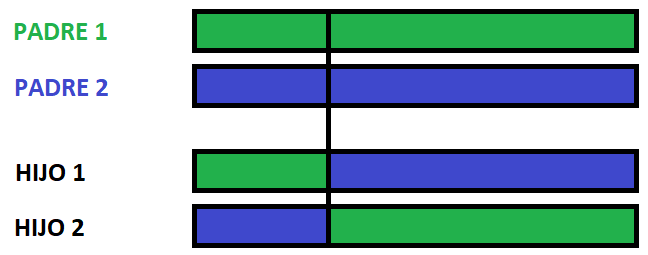
\includegraphics[scale=0.5]{imagenes/Crossover1point.png}
%%         \caption{$y=x$}
%         \label{fig:Crossover1point}
%     \end{subfigure}
%     \hfill
%     \begin{subfigure}[b]{0.3\textwidth}
%         \centering
%         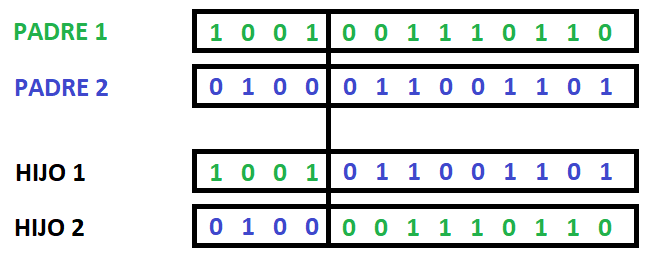
\includegraphics[scale=0.5]{imagenes/Crossover1pointNumber.png}
%%         \caption{$y=3\sin x$}
%         \label{fig:Crossover1pointNumber}
%     \end{subfigure}
		\centering
		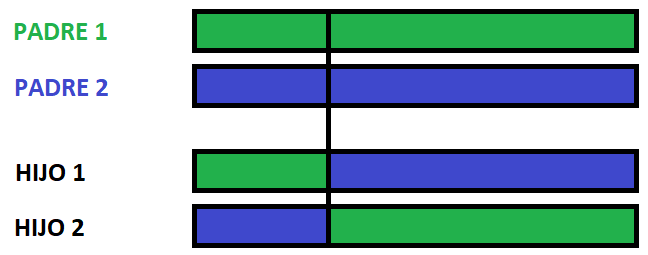
\includegraphics[scale=0.5]{imagenes/Crossover1point.png}
		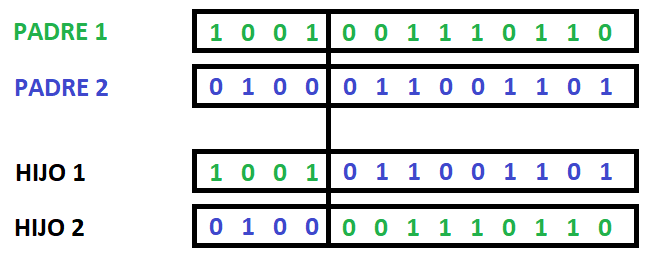
\includegraphics[scale=0.5]{imagenes/Crossover1pointNumber.png}
        \caption{Cruce en un punto}
        \label{fig:Crossover1}
\end{figure}

	\item \textbf{Cruce en dos puntos}: Sigue la misma lógica que el anterior, solo que elegimos dos puntos a partir de los cuales se cambian los elementos de qué padre se asignan a cada hijo. 
Un ejemplo de este tipo de cruce podría ser:
\begin{figure}[H]
		\centering
		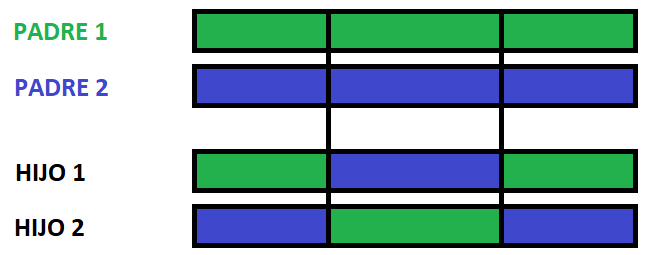
\includegraphics[scale=0.5]{imagenes/Crossover2point.png}
		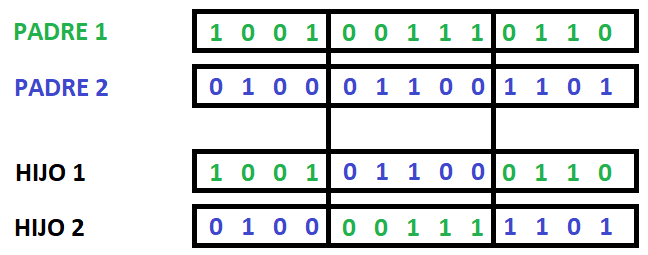
\includegraphics[scale=0.5]{imagenes/Crossover2pointNumber.png}
        \caption{Cruce en dos puntos}
        \label{fig:Crossover2}
\end{figure}
	\item \textbf{Cruce uniforme}: En este caso, en cada cromosoma se elige de forma aleatoria de qué padre lo hereda, cumpliéndose que si un hijo hereda cierto cromosoma de un padre, el otro hijo deberá heredar el mismo cromosoma del otro padre. 
Un ejemplo de este tipo de cruce sería: 
\begin{figure}[H]
		\centering
		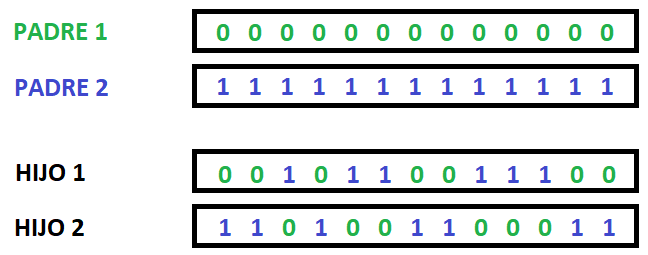
\includegraphics[scale=0.5]{imagenes/CrossoverUniformNumber.png}
        \caption{Cruce Uniforme}
        \label{fig:CrossoverUniform}
\end{figure}
\end{itemize}

El cruce de dos soluciones buenas no tiene por qué siempre dar lugar a una solución mejor o igual de buena. 
Sin embargo, si los padres son buenas soluciones, la probabilidad de tener un hijo bueno es elevada; en el caso de que el hijo no sea una buena solución, será eliminado durante el periodo de reemplazo. 

En nuestro problema es posible que el cruce de dos soluciones no de lugar a una solución. 
Esto se debe a la elección aleatoria de qué cromosomas elegir, no estamos teniendo en cuenta el peso que se está alcanzando al asignar cada elemento; por lo que es totalmente posible que  al asignar los elementos a cada hijo se sobrepase la capacidad máxima, dejando por ello de ser una solución válida. 

%Más adelante en este capítulo explicaremos otro tipo de cruce, que es el cruce HUX. 

En nuestro caso, realmente utilizamos una mezcla de cruce en un punto y cruce uniforme. 
Esto es, vamos a asignarle a cada hijo la mitad de cada uno de los padres, pero esta asignación será aleatoria: desordenamos el orden de los índices y lo partimos por la mitad. 
Esto viene representado en el pseudocódigo \ref{alg:CU}.

\begin{algorithm}
\caption{Cruce Uniforme}\label{alg:CU}
\begin{algorithmic}[1]
\Procedure \texttt{Cruce Uniforme}($padre_1, padre_2$)
\State Desordenar los índices que indican la posición de cada elemento
\For{i in 0..$n$}
	\If{i < $n/2$}
		\State \texttt{hijo$_1$[indice[i]]} = \texttt{padre$_1$[indice[i]]}
		\State \texttt{hijo$_2$[indice[i]]} = \texttt{padre$_2$[indice[i]]}
	\Else
		\State \texttt{hijo$_1$[indice[i]]} = \texttt{padre$_2$[indice[i]]}
		\State \texttt{hijo$_2$[indice[i]]} = \texttt{padre$_1$[indice[i]]}
	\EndIf
\EndFor
\EndProcedure
\end{algorithmic}
\end{algorithm}

\subsubsection{Mutación}

Los primeros intentos de mezclar computación y evolución no progresaron porque pusieron énfasis en los textos de biología del momento y confiaban más en la mutación que en el cruce para generar nuevas combinaciones de genes. 

La mutación consiste en modificar al azar una muy pequeña parte del cromosoma de los individuos, y permite alcanzar zonas del espacio de búsqueda que no estaban cubiertas por los individuos de la población actual. 
La mutación sola de por sí generalmente no permite avanzar en la búsqueda de una solución, pero nos garantiza que la población no va a evolucionar hacia una población uniforme que no sea capaz de seguir evolucionando. 

De forma similar a lo explicado en el Operador de Reparación, una vez que obtengamos la nueva solución debemos comprobar si podemos introducir más elementos, con el fin de maximizar el valor que puede llegar a tener. 
Esto también lo haremos siguiendo la misma lógica: ir introduciendo los genes con mayor proporción $valor\_acumulado/peso$. 

El pseudocódigo de nuestra implementación de la mutación viene expresada en Algoritmo \ref{alg:Mutation}. 

\begin{algorithm}
\caption{Mutación}\label{alg:Mutation}
\begin{algorithmic}[1]
\Procedure \texttt{Mutación}($poblacion$, $prob\_mut$)
\State Calcular el número de cromosomas que mutarán $\xrightarrow{}{}$ \texttt{nmut = $n$*prob\_mut}
\State Almacenar de forma aleatoria sin repetición \texttt{nmut} cromosomas de \texttt{poblacion} $\xrightarrow{}{}$\texttt{mutacion}
\For{i in 0..\texttt{nmut}}
	\State Elegir dos genes con distinto valor de forma aleatoria
	\If{Al intercambiar los genes sigue siendo válido}
		\State Intercambiar los genes
	\Else
		\State Volver al paso anterior
	\EndIf
	\State \texttt{anadido = true} 
	\While{\texttt{anadido}}
		\State \texttt{anadido} = Añadir elemento usando Greedy
	\EndWhile
	\State Calcular el valor de la función \textit{fitness}
\EndFor
\EndProcedure
\end{algorithmic}
\end{algorithm}

\subsubsection{Operador de Reemplazo Estacionario}

Una vez que hemos generado nuevas soluciones a partir del cruce de soluciones de la población existente, es necesario establecer un criterio sobre qué soluciones se mantienen o insertan en la población para la siguiente generación. 
En esta versión del Operador de Reemplazo el criterio que se sigue es el enfrentamiento de al población actual con las soluciones hijas, la población resultante estará compuesta de aquellos con mayor valor al calcular su función \textit{fitness}. 

En concreto, para lo que se aplica en el algoritmo base, AG, tenemos en cuenta que solo generamos 2 soluciones hijas antes de enfrentarlas con la población. 
Por ello, se ha optado por un método simplificado de enfrentamiento que consiste en encontrar cuáles son las 2 peores soluciones de la población actual (es decir, aquellas soluciones de la población actual con menor valor \textit{fitness}) y comprobar si las hijas son mejores o no. 
Se puede seguir su esquema en el pseudocódigo \ref{alg:ORE}. 
Usaremos los índices de forma que indique un orden de valores \textit{fitness}, por ejemplo, dados \texttt{padre$_1$} y  \texttt{padre$_2$}, se cumplirá que \textit{fitness}(\texttt{padre$_1$}) > \textit{fitness}(\texttt{padre$_2$}). 
Además, por conveniencia en la notación, se entenderá que \texttt{solucion$_i$} > \texttt{solucion$_j$} significa que el valor \textit{fitness} de \texttt{solucion$_i$} es mayor al de \texttt{solucion$_j$}.

Más adelante en la sección de ``Componentes de CHC'' de este capítulo se presenta la versión más generalizada de este tipo de enfrentamiento.

\begin{algorithm}
\caption{Operador de Reemplazo Estacionario}\label{alg:ORE}
\begin{algorithmic}[1]
\Procedure \texttt{Op Reemplazo Estacionario}
\State Calcular los 2 peores padres de la población actual $\xrightarrow{}{}$ \texttt{padre$_1$}, \texttt{padre$_2$}.
\If{\texttt{hijo$_1$} > \texttt{padre$_1$} \&\& \texttt{hijo$_2$} > \texttt{padre$_2$}}
	\State Intercambiar ambas soluciones de la población por ambos hijos
\ElsIf{\texttt{hijo$_1$} > \texttt{padre$_2$}}
	\State Intercambiar la peor solución de la población por el mejor hijo
\Else
	\State No hacer nada, ya que los dos hijos son peores que las peores soluciones de la población
\EndIf
\EndProcedure
\end{algorithmic}
\end{algorithm}

\section{CHC}

El algoritmo CHC utiliza un método de selección elitista que, combinada con un mecanismo de prevención de incesto y un método para obligar que la población diverja cada vez que converge, permite el mantenimiento de la diversidad de la población. 
Este algoritmo se ha utilizado de forma exitosa en el pasado para problemas de optimización estáticos. 

El algoritmo CHC (\textit{Cross-generational elitist selecition, Heterogeneous recombination and Cataclysmic mutation}) propuesto por Eshelman utiliza un método de selección elitista  combinado con un cruce altamente disruptivo para promover la diversidad de la población. 
La principal característica de este algoritmo es su capacidad de prevenir la convergencia de la población, algo que, como luego comprobaremos, será útil en nuestro problema. 

%En este algoritmo no se necesita de la mutación como era necesario en el AG, esto se debe precisamente a su característica principal, es capaz de forzar la diversidad de la población, por lo que la mutación deja de ser necesaria.

Originalmente, cuando la población converge se pueden tomar dos acciones:
\begin{itemize}
	\item Reiniciar la población entera de forma aleatoria con excepción de la mejor solución
	\item Reiniciar la población utilizando la mejor solución como base y generando el resto realizando modificaciones sobre esta.
\end{itemize}
Sin embargo, esto es solo útil cuando se tienen bastantes evaluaciones. 
En nuestro problema realizar esto resultaría en una pérdida de tiempo e iteraciones importantes, por lo tanto, no se tendrá en cuenta. 

\subsection{Pseudocódigo}

\begin{algorithm}
\caption{Algoritmo CHC}\label{alg:CHC}
\begin{algorithmic}[1]
\Procedure \texttt{AG}($EMax > 0, nelem > 0$)
\State Generar una población inicial aleatoria
\State Calcular la función \textit{fitness} de cada individuo
\State \texttt{generacion} = 0
\State \texttt{threshold} = $n$/4
\While{\texttt{generacion} < EMax}
	\State Calcular el número de parejas a formar para el cruce $\xrightarrow{}{} ncruce = pcruce*nelem$
	\State Desordenar los elementos de la población actual y comprobar si cumplen la condición de prevención de incesto (distancia de Hamming > \texttt{threshold}) de dos en dos
	\If{\texttt{hamming} > \texttt{threshold}}
		\State Almacenar las soluciones $\xrightarrow{}{}$ \texttt{parejas}
	\EndIf
	\If{\texttt{parejas} = $\emptyset$}
		\If{\texttt{threshold} $\neq$ 0}
			\State \texttt{threshold} = \texttt{threshold}-1
		\EndIf
	\Else
		\For{i$\in [0,\texttt{parejas.size()}]$; i=i+2}
			\State Generar 2 hijos cruzando \texttt{parejas}$[i]$ y \texttt{parejas}$[i+1]$
			\State Aplicar el Operador de Reparación sobre ambos hijos
			\State Calcular la función \textit{fitness} de cada hijo
			\State Almacenar dichos hijos $\xrightarrow{}{}$ \texttt{hijos}
		\EndFor
		\State Aplicar el Operador de Selección sobre la población actual e \texttt{hijos}
	\EndIf
	\State \texttt{generacion} = \texttt{generacion}+1
\EndWhile
\EndProcedure
\end{algorithmic}
\end{algorithm}

\subsection{Componentes}
\subsubsection{Operador de reparación}
Se utilizará el mismo que se ha presentado anteriormente en los componentes de AG. 
Véase el pseudocódigo \ref{alg:OR}.

\subsubsection{Cruce HUX}

El cruce HUX (\textit{Half Uniform Crossover}) se caracteriza por, dados dos cromosomas, asignarle a los resultados del cruce en primer lugar los genes comunes a ambos padres y el resto de los genes serán repartidos a partes iguales entre ambos padres. 
Es decir, exactamente la mitad de los genes no coincidentes se intercambian en los hijos. 

A continuación se detallará en forma de pseudocódigo (\ref{alg:HUX}) el comportamiento de este tipo de cruce. 
Aunque primero se mostrará un ejemplo de este tipo de cruce en Figura \ref{fig:HUX}.

\begin{figure}
		\centering
		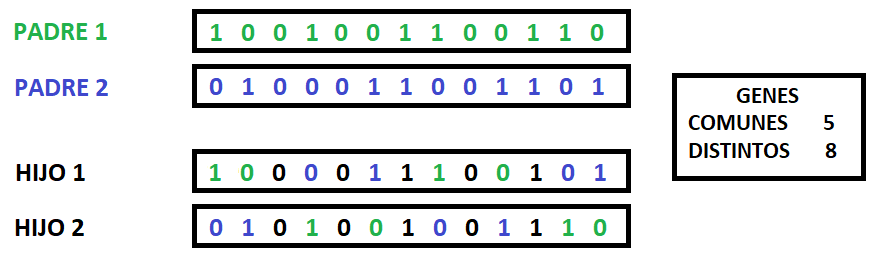
\includegraphics[scale=0.5]{imagenes/CrossoverHUX.png}
        \caption{Cruce HUX}
        \label{fig:HUX}
\end{figure}

\begin{algorithm}
\caption{Cruce HUX}\label{alg:HUX}
\begin{algorithmic}[1]
\Procedure \texttt{Cruce HUX}($padre_1, padre_2$)
\State Asignar los genes comunes de los padres a ambos hijos
\State Desordenar los índices que indican la posición de cada gen restante $\xrightarrow{}{}$ Supongamos tamaño $m \leq n$
\For{i in 0..$m$}
	\If{i < $m/2$}
		\State \texttt{hijo$_1$[indice[i]]} = \texttt{padre$_1$[indice[i]]}
		\State \texttt{hijo$_2$[indice[i]]} = \texttt{padre$_2$[indice[i]]}
	\Else
		\State \texttt{hijo$_1$[indice[i]]} = \texttt{padre$_2$[indice[i]]}
		\State \texttt{hijo$_2$[indice[i]]} = \texttt{padre$_1$[indice[i]]}
	\EndIf
\EndFor
\EndProcedure
\end{algorithmic}
\end{algorithm}

\subsubsection{Enfrentamiento}

Es una generalización del Operador de Reemplazo Estacionario del AG (Algoritmo \ref{alg:ORE}). 
En este caso tenemos que enfrentar toda la población de hijos (con tamaño menor igual al tamaño de la población) contra toda la generación anterior. 
Por ello, no podemos seguir el método de obtener los $x$ peores elementos de la población para enfrentarlos con los hijos; así que optaremos por otro razonamiento. 

Se ha optado por, a grandes rasgos, juntar ambas poblaciones (generación actual y descendientes) en una sola y ordenarlas en base a su valor \textit{fitness}. 
De esta forma, al final	tenemos todas nuestras soluciones ordenadas de mejor a peor y solo tenemos que quedarnos con las $n$ para formar la nueva población. 

Este comportamiento se puede ver reflejado en su pseudocódigo (Algoritmo \ref{alg:Enfrentamiento})

\begin{algorithm}[H]
\caption{Enfrentamiento CHC}\label{alg:Enfrentamiento}
\begin{algorithmic}[1]
\Procedure \texttt{Enfrentamiento}($poblacion, hijos$)
\State Calcular la función \textit{fitness} de \texttt{poblacion} e \texttt{hijos}
\State Unir ambas poblaciones $\xrightarrow{}{}$ \texttt{pobTotal}
\State Unir los valores de ambas poblaciones $\xrightarrow{}{}$ \texttt{valorTotal} 
\State Ordenar los elementos de \texttt{pobTotal} según \texttt{valorTotal} (orden descendente)
\State Asignar a la población actual los $n$ primeros elementos de \texttt{pobTotal}
\EndProcedure
\end{algorithmic}
\end{algorithm}
